\documentclass[12pt, letterpaper]{article}

% --- PACKAGES ---
\usepackage[utf8]{inputenc}
\usepackage[T1]{fontenc}
\usepackage{mathpazo} % Palatino Font
\usepackage[margin=1in]{geometry}
\usepackage{amsmath, amssymb, amsfonts, amsthm}
\usepackage{mathtools}
\usepackage{fancyhdr} 
\usepackage{xcolor}
\usepackage{tikz} 
\usetikzlibrary{arrows.meta, calc}
\usepackage[most]{tcolorbox} 

% --- CUSTOM MACROS ---
\newcommand{\RR}{\mathbb{R}}
\newcommand{\CC}{\mathbb{C}}
\newcommand{\dd}{\mathrm{d}}
\newcommand{\p}{\partial}
\newcommand{\wedgeprod}{\wedge}

% --- COLORS & STYLE ---
\definecolor{themecolor}{RGB}{0, 51, 102} % Navy Blue
%\definecolor{gray}{gray} 

% --- PAGE HEADER/FOOTER ---
\pagestyle{fancy}
\fancyhf{}
\fancyhead[L]{\small \textsc{Vector Calculus \& Complex Forms}}
\fancyhead[R]{\small \today}
\fancyfoot[C]{\thepage}
\renewcommand{\headrulewidth}{0.4pt}

% --- NOTE BOX COMMAND ---
% Usage: \makenote{Title}{Content}
\newcounter{notecount}
\newcommand{\makenote}[2]{
	\clearpage
	\stepcounter{notecount}
	
	% The Content Box
	\begin{tcolorbox}[
		enhanced,
		colback=white,
		colframe=themecolor,
		coltitle=white,
		fonttitle=\bfseries\Large,
		title={Topic \thenotecount: #1},
		sharp corners=south,
		drop fuzzy shadow,
		boxrule=0.5mm,
		top=6mm, bottom=6mm
		]
		\large #2
	\end{tcolorbox}
	
	% The Workspace (Fine Line Grid)
	\vfill
	\begin{center}
		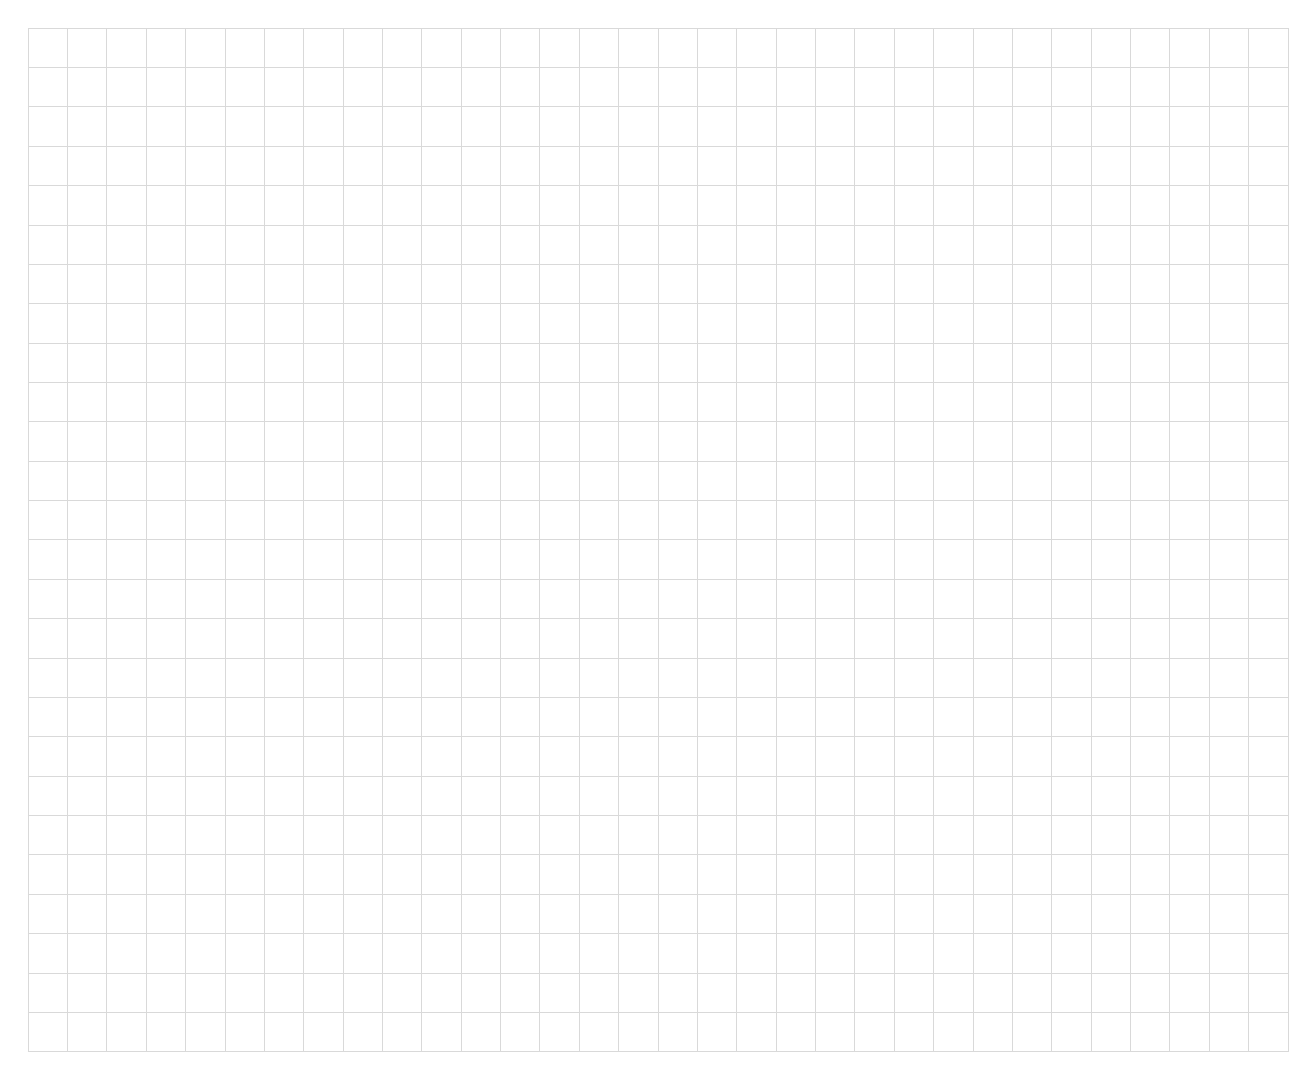
\begin{tikzpicture}
			% step=0.5cm, line width=0.2pt, very light gray
			\draw[step=0.5cm, gray!30, line width=0.2pt] (0,0) grid (16,13);
		\end{tikzpicture}
	\end{center}
	\vfill
}

% --- TITLE PAGE ---
\title{
	\vspace{2cm}
	\begin{tcolorbox}[colback=themecolor, colframe=themecolor, sharp corners]
		\centering \color{white}
		\Huge \textbf{Mathematical Methods}\\
		\vspace{0.5em}
		\Large \textit{From Vector Calculus to Differential Forms}
	\end{tcolorbox}
}
\author{\textbf{Lecture Notes \& Practice}}
\date{\today}

% --- DOCUMENT START ---
\begin{document}
	
	\begin{titlepage}
		\centering
		\maketitle
		\thispagestyle{empty}
		
		\vspace{2cm}
		
		% TikZ Visualization: Stokes' Theorem Concept
		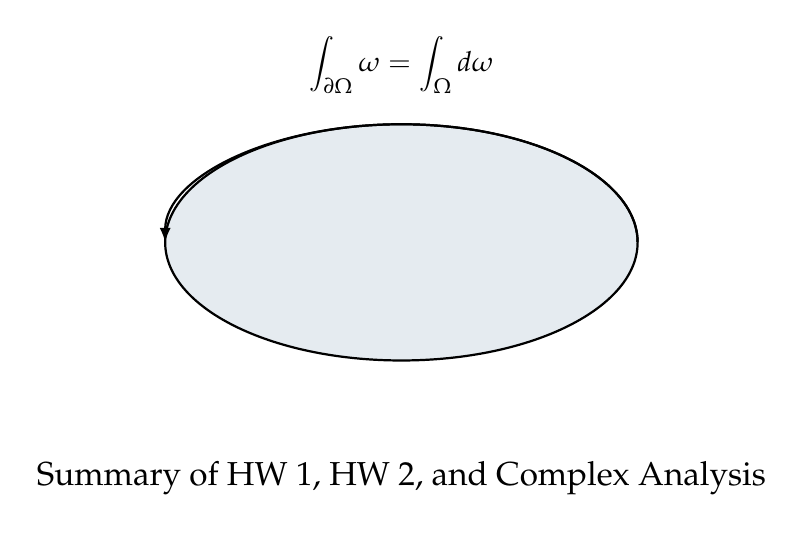
\begin{tikzpicture}[scale=1.5]
			\draw[thick, fill=themecolor!10] (0,0) ellipse (2cm and 1cm);
			\draw[thick, ->, >=latex] (2,0) arc (0:180:2cm and 1cm);
			\node at (0, 1.5) {$\displaystyle \int_{\partial \Omega} \omega = \int_{\Omega} d\omega$};
			\node at (0, -2) {\large Summary of HW 1, HW 2, and Complex Analysis};
		\end{tikzpicture}
	\end{titlepage}
	
	% --- TOPIC 1: LINE INTEGRALS ---
	\makenote{Line Integrals of Vector Fields}{
		Given a curve $\gamma: [a, b] \to \RR^2$ and a vector field $\mathbf{F}$ defined on a neighborhood of $\gamma$, the line integral is defined as:
		$$ \int_{\gamma} \mathbf{F} \cdot \dd \gamma = \int_{a}^{b} \mathbf{F}(\gamma(t)) \cdot \gamma'(t) \, \dd t $$
		
		\textbf{Example (The Vortex Field):} 
		Consider $\mathbf{F}(x,y) = \left( -\frac{y}{x^2+y^2}, \frac{x}{x^2+y^2} \right)$.
		Calculate $\int_C \mathbf{F} \cdot \dd \mathbf{r}$ where $C$ is the unit circle traversed counter-clockwise.
		
		\textit{(Space below for derivation showing the result is $2\pi$)}
	}
	
	% --- TOPIC 2: SURFACE INTEGRALS ---
	\makenote{Surface Integrals and Flux}{
		Let $S$ be a surface parametrized by $T(u,v)$. The surface integral of a vector field $\mathbf{F}$ uses the outward normal vector $\mathbf{N} = T_u \times T_v$:
		$$ \iint_{S} \mathbf{F} \cdot \dd S := \iint_{D} \mathbf{F}(T(u,v)) \cdot \left( \frac{\p T}{\p u} \times \frac{\p T}{\p v} \right) \dd A $$
		
		\textbf{Exercise:} Compute the flux for $\mathbf{F}=(x,y,-z)$ over a parametrized surface $S$.
	}
	
	% --- TOPIC 3: STOKES' THEOREM OBSERVATION ---
	\makenote{Stokes' Theorem \& Surface Independence}{
		Consider the vector field $\mathbf{F} = (y, xz, 1)$. We observe that $\iint_S \mathrm{curl}\,\mathbf{F} \cdot \dd S$ yields the \textbf{same result} for:
		\begin{enumerate}
			\item The Disk ($x^2+y^2 \le 1, z=0$)
			\item The Hemisphere ($x^2+y^2+z^2=1, z \ge 0$)
			\item The Paraboloid ($z = 1-x^2-y^2, z \ge 0$)
		\end{enumerate}
		Why? Because they share the same boundary $\partial S$. This is the essence of Stokes' Theorem:
		$$ \iint_S (\nabla \times \mathbf{F}) \cdot \dd S = \oint_{\partial S} \mathbf{F} \cdot \dd \mathbf{r} $$
	}
	
	% --- TOPIC 4: DIFFERENTIAL FORMS ---
	\makenote{Exterior Derivative \& Differential Forms}{
		A $k$-form is an object that can be integrated over a $k$-dimensional manifold.
		\begin{itemize}
			\item \textbf{0-form:} Smooth function $f$. $df = \sum \frac{\p f}{\p x_i} \dd x_i$.
			\item \textbf{1-form:} $\omega = \sum a_i \dd x_i$. 
			\item \textbf{Exterior Derivative:} $d\omega$ maps $k$-forms to $(k+1)$-forms.
		\end{itemize}
		\textbf{Property:} $d(d\omega) = 0$. This generalizes $\mathrm{curl}(\nabla f)=0$ and $\mathrm{div}(\mathrm{curl}\,\mathbf{F})=0$.
		
		\textbf{Exercise:} Compute $d\eta$ for $\eta = P \dd x + Q \dd y + R \dd z$.
	}
	
	% --- TOPIC 5: COMPLEXIFICATION ---
	\makenote{Complex Forms \& The Cauchy-Green Formula}{
		We can relate real 1-forms to complex differentials ($z = x+iy, \dd z = \dd x + i \dd y$).
		
		The "Vortex Field" $\mathbf{F} = (-y/r^2, x/r^2)$ corresponds to the 1-form:
		$$ \omega = \frac{-y \dd x + x \dd y}{x^2+y^2} = \mathrm{Im}\left( \frac{\dd z}{z} \right) $$
		
		This connects vector calculus to the Cauchy Integral Formula:
		$$ \int_C \frac{1}{z} \dd z = 2\pi i $$
		\textit{(Derive the relationship between the real line integral and the complex contour integral below)}
	}
	
\end{document}